\section{目的}
% コード生成とはプログラムを生成する段階や,生成したプログラムを実行する段階など,複 数のステージを持つプログラミングの手法である.プログラムを計算対象のデータとして扱 うことで,プログラムの効率や,保守性,再利用性 の両立が期待できる.例えば生成元のプ ログラムから,何らかの目的に特化したプログラムを生成を行い,保守や改変をしたい時は, 生成元のプログラムに対して行えばよいので,生成後のコードについては手を加える必要が 無い.そのようなコード生成を効果的に行うためには,言語レベルで,プログラムを生成,実 行などを行う機構を備えることが望ましい.そのような言語をコード生成言語という.

\begin{frame}
  \frametitle{目的}
  % \blue{コード生成の説明と,研究の目的を同時に話す}
  % \vspace{-4zh} %% odd
  \medskip
  \flushleft
  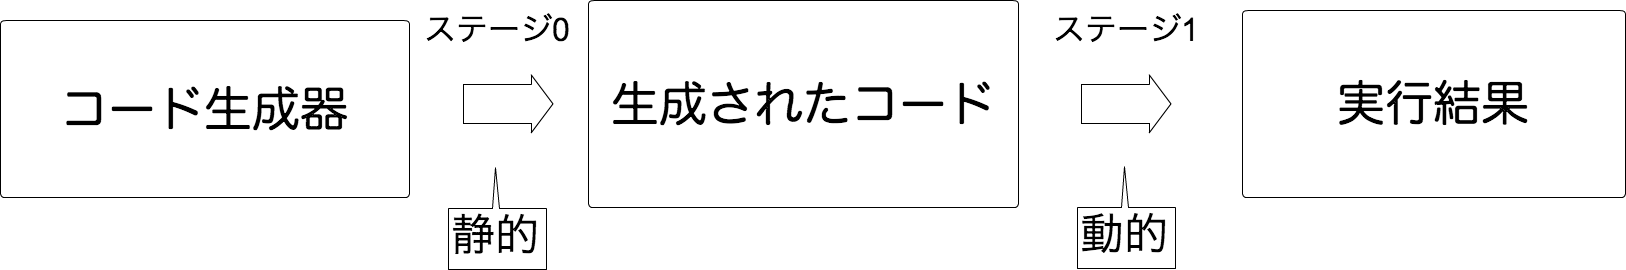
\includegraphics[clip,height=2cm]{./img/prggen.png}

  \begin{itemize}
    % \item コード生成ステージとコード実行ステージ
    % \item 生成前の段階で,生成後のコードの安全性を保証する
  \item コード生成をサポートするプログラム言語\\(=\alert{コード生成言語})
    % \item[◯]<2-> 生成するプログラムだけでなく,生成されたプログラムも型の整合性が静的に (生成前に) 保証される
  \end{itemize}

  \begin{visibleenv}<2>
    \begin{block}{\textbf{表現力}と\textbf{安全性}を兼ね備えたコード生成言語の構築}
      \begin{itemize}
      \item 表現力: 多段階let挿入,メモ化等の技法を表現
      \item 安全性: 生成されるコードの一定の性質を静的に検査
      \end{itemize}
    \end{block}
  \end{visibleenv}

\end{frame}

\begin{frame}
  \frametitle{コード生成前に型付け,生成後のコードの型安全性を保証}
  % \begin{onlyenv}<1>
  %   \center
  %   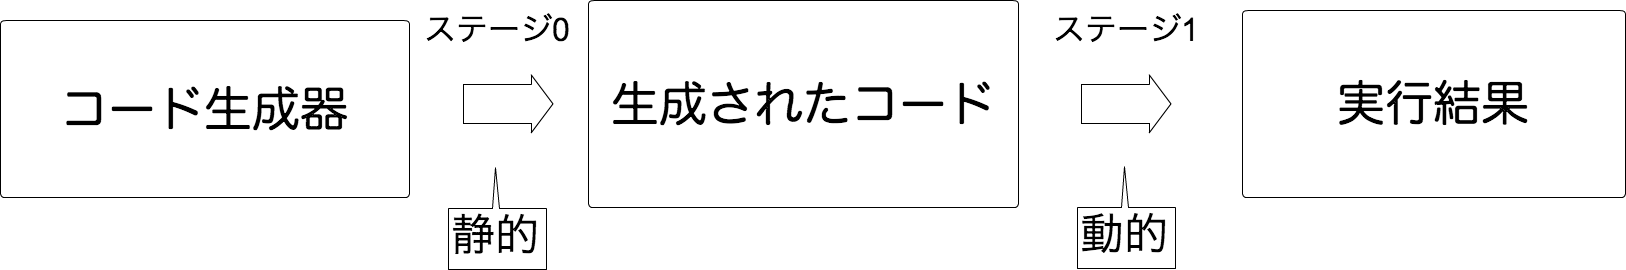
\includegraphics[clip,height=1.9cm]{./img/prggen.png}
  % \end{onlyenv}

  % \begin{onlyenv}<2>
  %   \center
  %   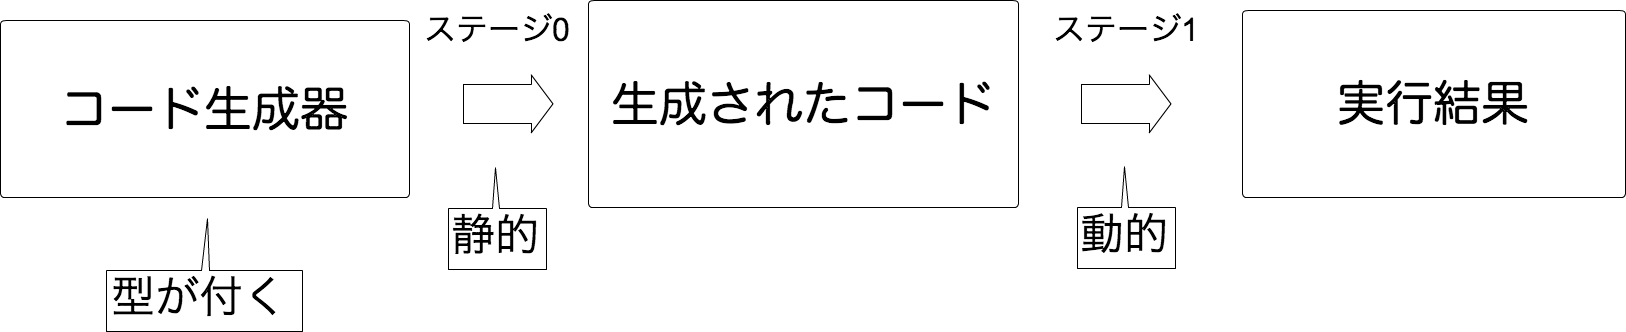
\includegraphics[clip,height=2.4cm]{./img/prggen_type1.png}
  % \end{onlyenv}

  % \begin{onlyenv}<3>
  %   \center
  %   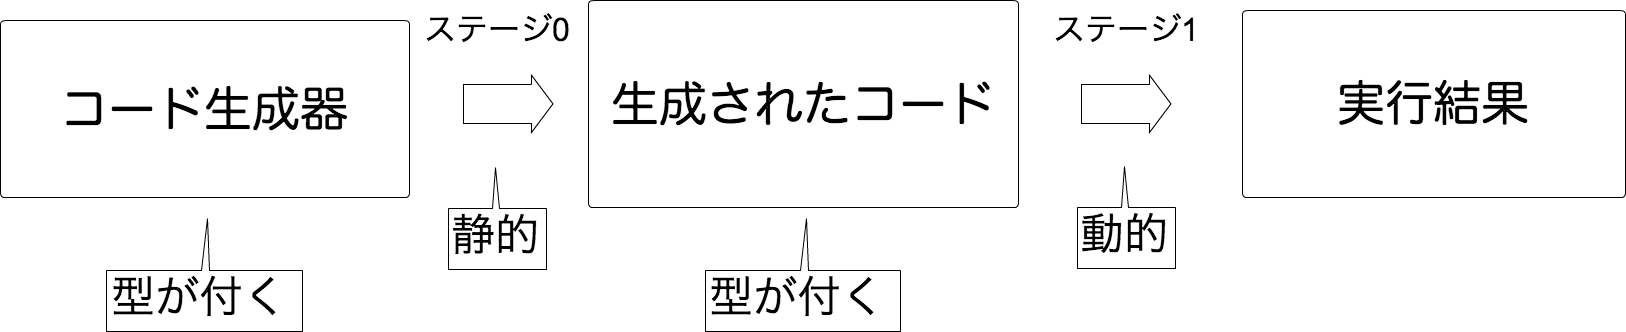
\includegraphics[clip,height=2.4cm]{./img/prggen_type2.png}
  % \end{onlyenv}

  % \begin{onlyenv}<4>
  %   \center
  %   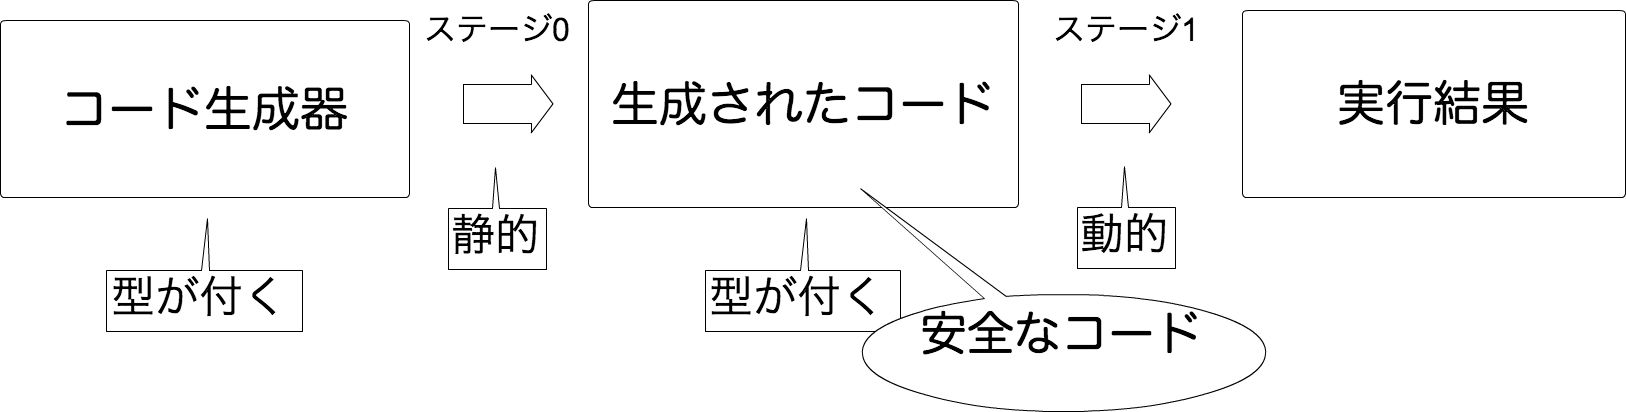
\includegraphics[clip,height=3.0cm]{./img/prggen_type3.png}
  % \end{onlyenv}

  \begin{onlyenv}<1->
    \center
    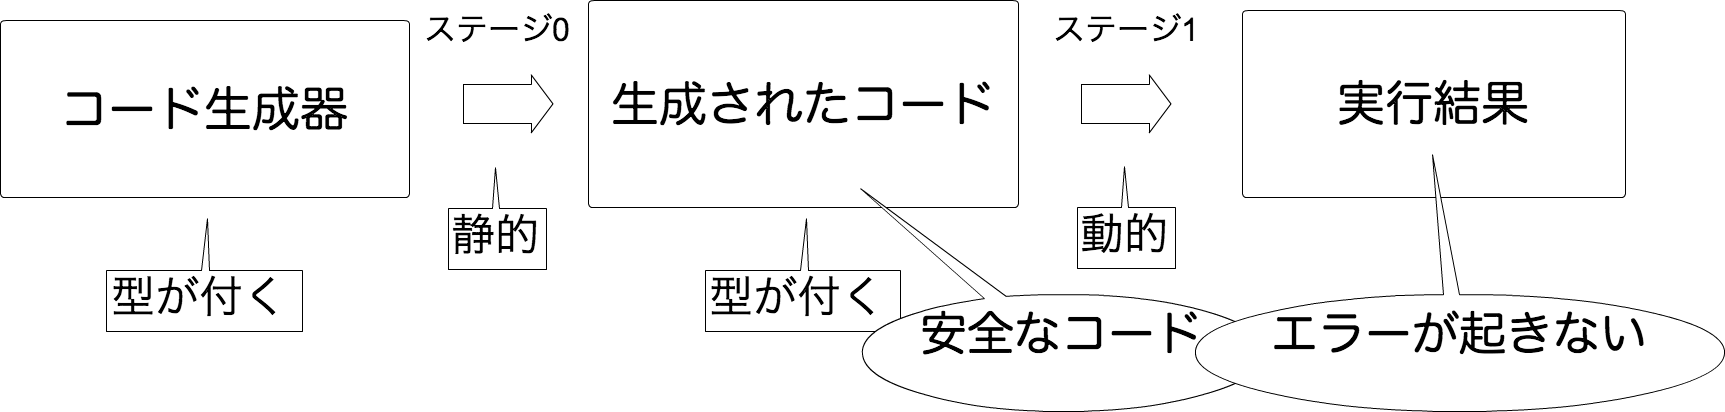
\includegraphics[clip,height=3.0cm]{./img/prggen_type4.png}
  \end{onlyenv}

  \begin{uncoverenv}<2>
    \begin{block}{本研究: 簡潔で強力なコントロールオペレータに基づくコード生成体系の構築}
      \begin{itemize}
      \item コントロールオペレータ shift0/reset0 を利用し,多段階let挿入などのコード生成技法を表現
      \item 型システムを構築して型安全性を保証
      \end{itemize}
    \end{block}
  \end{uncoverenv}

\end{frame}

% \section{研究の目的}
% \begin{frame}
%   \frametitle{研究の目的}

%   \begin{block}{\textbf{表現力}と\textbf{安全性}を兼ね備えたコード生成言語の構築}
%     \begin{itemize}
%     \item 表現力: 多段階let挿入,メモ化等の技法を表現
%     \item 安全性: 生成されるコードの一定の性質を静的に検査
%     \end{itemize}
%   \end{block}

%   \medskip
%   \pause

%   \begin{block}{本研究: 簡潔で強力なコントロールオペレータに基づくコード生成体系の構築}
%     \begin{itemize}
%     \item コントロールオペレータ shift0/reset0 を利用し,let挿入などのコード生成技法を表現
%     \item 型システムを構築して型安全性を保証
%     \end{itemize}
%   \end{block}
% \end{frame}

% \section{研究の内容}

% \begin{frame}
%   \center
%   \huge{表現力を上げ(コードレベルでの多段階let挿入),安全性も保証するためにどうすればよいのか}
% \end{frame}


%%% Local Variables:
%%% mode: latex
%%% TeX-master: "slide_oishi"
%%% End:
